\documentclass{article}
\usepackage[utf8]{inputenc}
\usepackage[english]{babel}

\usepackage{xcolor}
\def\pgfsysdriver{pgfsys-ximera.def}
\usepackage{tikz}

\begin{document}

This example shows different examples on how to use the \texttt{xcolor} package 
to change the colour of elements in \LaTeX.

\begin{itemize}
\color{blue}
\item First item
\item Second item
\end{itemize}

\noindent
{\color{red} \rule{\linewidth}{0.5mm} }
\newpage

\begin{itemize}
\color{green}
\item First item
\item Second item
\end{itemize}
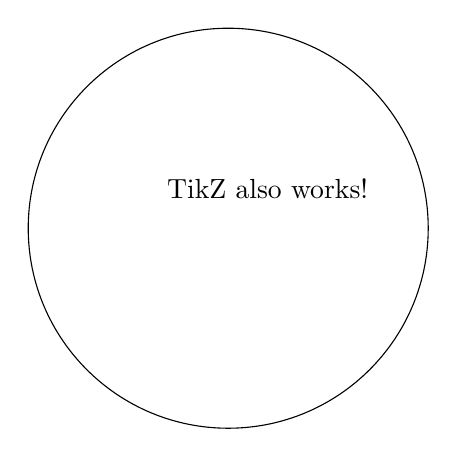
\begin{tikzpicture}                                                             
  \draw (0,0) circle (1in);                                                       
  \node at (0.5,0.5) (x) {TikZ also works!};                                      
\end{tikzpicture}  

\end{document}
